% ------------------------------------------------------------------------------
\subsection{Tables of Upper Limits for the Search for Resonant \HH Production}%
\label{app:limit_tables}
% ------------------------------------------------------------------------------

{
  \centering

  \vspace*{1em}

  \captionof{table}[Expected and observed upper limits on
  $\sigma(\pp \to X \to \HH)$ for the combination of all channels.]{Expected and
    observed upper limits on the cross section of $\pp \to X \to \HH$ at
    \SI{95}{\percent}~CL for the combination of all channels.}%
  \label{tab:comb_limits_resonant}

  % Workspaces: comb_2022_01_29
  \setlength{\tabcolsep}{1.2em}

\begin{tabular}{
  S[round-mode=places, round-precision=1, table-format=4.0]
  S[round-mode=figures, round-precision=2, table-format=4.0]
  S[round-mode=figures, round-precision=2, table-format=4.1]
  S[round-mode=figures, round-precision=2, table-format=4.1]
  S[round-mode=figures, round-precision=2, table-format=4.1]
  S[round-mode=figures, round-precision=2, table-format=4.1]
  S[round-mode=figures, round-precision=2, table-format=4.1]
  }
  \toprule
  & \multicolumn{6}{c}{Upper limit on $\sigma(\pp \to X \to \HH)$ at \SI{95}{\percent}~CL / \si{\femto\barn}} \\ \cmidrule{2-7}
  {$\mX / \si{\GeV}$} & {Observed} & {-2$\sigma$} & {-1$\sigma$} & {Expected} & {+1$\sigma$} & {+2$\sigma$} \\
  \midrule
  251 & 638.439474 &   181.597753 &   243.795325 & 338.343637 &   470.876453 &   631.243225 \\
  260 & 896.941144 &   388.414694 &   521.447460 & 723.674376 &  1007.145358 &  1350.149661 \\
  280 & 486.649582 &   451.329066 &   605.910122 & 840.893212 &  1170.280064 &  1568.843286 \\
  300 & 536.855730 &   354.268351 &   475.605929 & 660.054657 &   918.605115 &  1231.455197 \\
  325 & 335.203789 &   253.311729 &   340.071473 & 471.957446 &   656.828218 &   880.524732 \\
  350 & 225.955597 &   188.434655 &   252.973879 & 351.081802 &   488.604294 &   655.008651 \\
  375 & 128.478432 &   116.329338 &   156.172355 & 216.738867 &   301.637796 &   404.366822 \\
  400 &  79.740112 &    76.742967 &   103.027578 & 142.983568 &   198.991758 &   266.762541 \\
  450 &  47.487654 &    36.311632 &    48.748434 &  67.653973 &    94.154757 &   126.221118 \\
  500 &  46.443591 &    22.921119 &    30.771645 &  42.705456 &    59.433639 &    79.675001 \\
  550 &  25.460027 &    17.653045 &    23.699246 &  32.890250 &    45.773712 &    61.362902 \\
  600 &  21.061634 &    14.051405 &    18.864037 &  26.179858 &    36.434787 &    48.843412 \\
  700 &  25.438956 &    10.020276 &    13.452240 &  18.669266 &    25.982217 &    34.831001 \\
  800 &  30.810426 &     8.174691 &    10.974539 &  15.230667 &    21.196681 &    28.415652 \\
  900 &  30.585851 &     7.193141 &     9.656806 &  13.401892 &    18.651557 &    25.003732 \\
  1000 &  30.462079 &     6.544590 &     8.786125 &  12.193545 &    16.969887 &    22.749335 \\
  1100 &  27.986994 &     7.199577 &     9.665446 &  13.413883 &    18.668245 &    25.026104 \\
  1200 &  24.592590 &     7.380353 &     9.908137 &  13.750695 &    19.136990 &    25.654490 \\
  1400 &  27.352079 &    10.649380 &    14.296812 &  19.841379 &    27.613459 &    37.017797 \\
  1600 &  33.882981 &    16.663186 &    22.370359 &  31.045995 &    43.207043 &    57.922100 \\
  \bottomrule
\end{tabular}

%%% Local Variables:
%%% mode: latex
%%% TeX-master: "../phd_thesis"
%%% End:

}

\clearpage

{
  \centering

  \null\vfill

  \captionof{table}[Expected and observed upper limits on
  $\sigma(\pp \to X \to \HH)$ for the combination of the \hadhad channel and
  the \ZHF~CR.]{Expected and observed upper limits on the cross section of
    $\pp \to X \to \HH$ at \SI{95}{\percent}~CL for the combination of the \hadhad
    channel and the \ZHF~CR.}%
  \label{tab:hadhad_limits_resonant}

  % Workspaces: comb_2022_01_29
  \setlength{\tabcolsep}{1.2em}

\begin{tabular}{
  S[round-mode=places, round-precision=1, table-format=4.0]
  S[round-mode=figures, round-precision=2, table-format=4.0]
  S[round-mode=figures, round-precision=2, table-format=4.1]
  S[round-mode=figures, round-precision=2, table-format=4.1]
  S[round-mode=figures, round-precision=2, table-format=4.1]
  S[round-mode=figures, round-precision=2, table-format=4.1]
  S[round-mode=figures, round-precision=2, table-format=4.1]
  }
  \toprule
  & \multicolumn{6}{c}{Upper limit on $\sigma(\pp \to X \to \HH)$ at \SI{95}{\percent}~CL / \si{\femto\barn}} \\ \cmidrule{2-7}
  {$\mX / \si{\GeV}$} &  {Observed} & {-2$\sigma$} & {-1$\sigma$} &  {Expected} & {+1$\sigma$} & {+2$\sigma$} \\
  \midrule
  251 &  973.495799 &   265.045066 &   355.823501 &  493.818400 &   687.252341 &   921.310423 \\
  260 & 1627.925794 &   557.380325 &   748.284137 & 1038.482489 &  1445.267171 &  1937.482972 \\
  280 &  885.081013 &   554.703191 &   744.690080 & 1033.494591 &  1438.325460 &  1928.177118 \\
  300 &  900.688379 &   426.880001 &   573.087206 &  795.340965 &  1106.884516 &  1483.857065 \\
  325 &  427.179604 &   285.774280 &   383.652509 &  532.440009 &   741.002448 &   993.366246 \\
  350 &  262.632595 &   216.567956 &   290.742890 &  403.498330 &   561.552936 &   752.801470 \\
  375 &  153.878061 &   126.844843 &   170.289441 &  236.330819 &   328.904125 &   440.919267 \\
  400 &  102.277962 &    84.818611 &   113.869145 &  158.029694 &   219.931613 &   294.833899 \\
  450 &   62.479143 &    41.225854 &    55.345787 &   76.809901 &   106.897159 &   143.303211 \\
  500 &   55.685134 &    28.092274 &    37.713931 &   52.340087 &    72.842259 &    97.650205 \\
  550 &   25.524188 &    21.202297 &    28.464123 &   39.503034 &    54.976794 &    73.700285 \\
  600 &   26.608906 &    17.384295 &    23.338449 &   32.389529 &    45.076853 &    60.428713 \\
  700 &   32.164818 &    12.811085 &    17.198906 &   23.868959 &    33.218685 &    44.531999 \\
  800 &   33.258635 &    10.820855 &    14.527018 &   20.160863 &    28.058088 &    37.613854 \\
  900 &   42.358711 &     9.759847 &    13.102613 &   18.184048 &    25.306933 &    33.925736 \\
  1000 &   43.661054 &     9.557592 &    12.831085 &   17.807216 &    24.782492 &    33.222686 \\
  1100 &   35.580690 &    10.783233 &    14.476511 &   20.090768 &    27.960536 &    37.483079 \\
  1200 &   35.027829 &    11.710499 &    15.721367 &   21.818402 &    30.364903 &    40.706303 \\
  1400 &   34.671442 &    16.796855 &    22.549810 &   31.295041 &    43.553643 &    58.386742 \\
  1600 &   38.223685 &    24.965885 &    33.516747 &   46.515158 &    64.735643 &    86.782712 \\
  \bottomrule
\end{tabular}

%%% Local Variables:
%%% mode: latex
%%% TeX-master: "../phd_thesis"
%%% End:


  \null\vfill
}

\clearpage

{
  \centering

  \null\vfill

  \captionof{table}[Expected and observed upper limits on
  $\sigma(\pp \to X \to \HH)$ for the combination of the \lephad channels and
  the \ZHF~CR.]{Expected and observed upper limits on the cross section of
    $\pp \to X \to \HH$ at \SI{95}{\percent}~CL for the combination of the
    \lephad channels and the \ZHF~CR.}%
  \label{tab:lephad_limits_resonant}

  % Workspaces: comb_2022_01_29
  \setlength{\tabcolsep}{1.2em}

\begin{tabular}{
  S[round-mode=places, round-precision=1, table-format=4.0]
  S[round-mode=figures, round-precision=2, table-format=4.0]
  S[round-mode=figures, round-precision=2, table-format=4.1]
  S[round-mode=figures, round-precision=2, table-format=4.1]
  S[round-mode=figures, round-precision=2, table-format=4.1]
  S[round-mode=figures, round-precision=2, table-format=4.1]
  S[round-mode=figures, round-precision=2, table-format=4.1]
  }
  \toprule
  & \multicolumn{6}{c}{Upper limit on $\sigma(\pp \to X \to \HH)$ at \SI{95}{\percent}~CL / \si{\femto\barn}} \\ \cmidrule{2-7}
  {$\mX / \si{\GeV}$} & {Observed} & {-2$\sigma$} & {-1$\sigma$} &  {Expected} & {+1$\sigma$} & {+2$\sigma$} \\
  \midrule
  251 & 588.078287 &   270.267317 &   362.834383 &  503.548230 &   700.793450 &   939.463238 \\
  260 & 824.081799 &   565.705702 &   759.460971 & 1053.993905 &  1466.854575 &  1966.422415 \\
  280 & 651.466985 &   730.921391 &   981.263345 & 1361.815320 &  1895.252925 &  2540.720736 \\
  300 & 698.905380 &   655.009622 &   879.351652 & 1220.380397 &  1698.416433 &  2276.847481 \\
  325 & 711.861349 &   547.597703 &   735.150949 & 1020.256009 &  1419.901184 &  1903.478071 \\
  350 & 624.218886 &   412.157831 &   553.322665 &  767.911372 &  1068.710458 &  1432.682037 \\
  375 & 420.188007 &   329.901484 &   442.893364 &  614.655557 &   855.422703 &  1146.754700 \\
  400 & 228.387428 &   207.288383 &   278.285045 &  386.209104 &   537.491335 &   720.545191 \\
  450 & 113.768039 &    85.078354 &   114.217850 &  158.513633 &   220.605116 &   295.736778 \\
  500 &  85.822225 &    45.593490 &    61.209346 &   84.947456 &   118.222282 &   158.485339 \\
  550 &  77.734239 &    36.599274 &    49.134594 &   68.189894 &    94.900603 &   127.220978 \\
  600 &  42.243468 &    27.557005 &    36.995331 &   51.342801 &    71.454324 &    95.789581 \\
  700 &  36.181132 &    18.514322 &    24.855513 &   34.494938 &    48.006973 &    64.356747 \\
  800 &  42.778225 &    14.277970 &    19.168202 &   26.601983 &    37.022264 &    49.630967 \\
  900 &  29.078821 &    12.077263 &    16.213748 &   22.501738 &    31.315910 &    41.981194 \\
  1000 &  28.091234 &    10.168604 &    13.651371 &   18.945623 &    26.366826 &    35.346597 \\
  1100 &  32.580898 &    10.354839 &    13.901391 &   19.292607 &    26.849727 &    35.993960 \\
  1200 &  27.175534 &    10.332595 &    13.871528 &   19.251162 &    26.792047 &    35.916636 \\
  1400 &  38.599101 &    15.186587 &    20.388022 &   28.294871 &    39.378275 &    52.789365 \\
  1600 &  61.138650 &    24.627287 &    33.062179 &   45.884300 &    63.857670 &    85.605728 \\
  \bottomrule
\end{tabular}

%%% Local Variables:
%%% mode: latex
%%% TeX-master: "../phd_thesis"
%%% End:


  \null\vfill
}


% ------------------------------------------------------------------------------
\clearpage
\subsection{Post-Fit Distributions of PNN Discriminants in the \lephad
  Channels}%
\label{app:pnn_plots_lephad}
% ------------------------------------------------------------------------------

\begin{figure}[htbp]
  \centering

  \begin{subfigure}{0.495\textwidth}
    \centering

    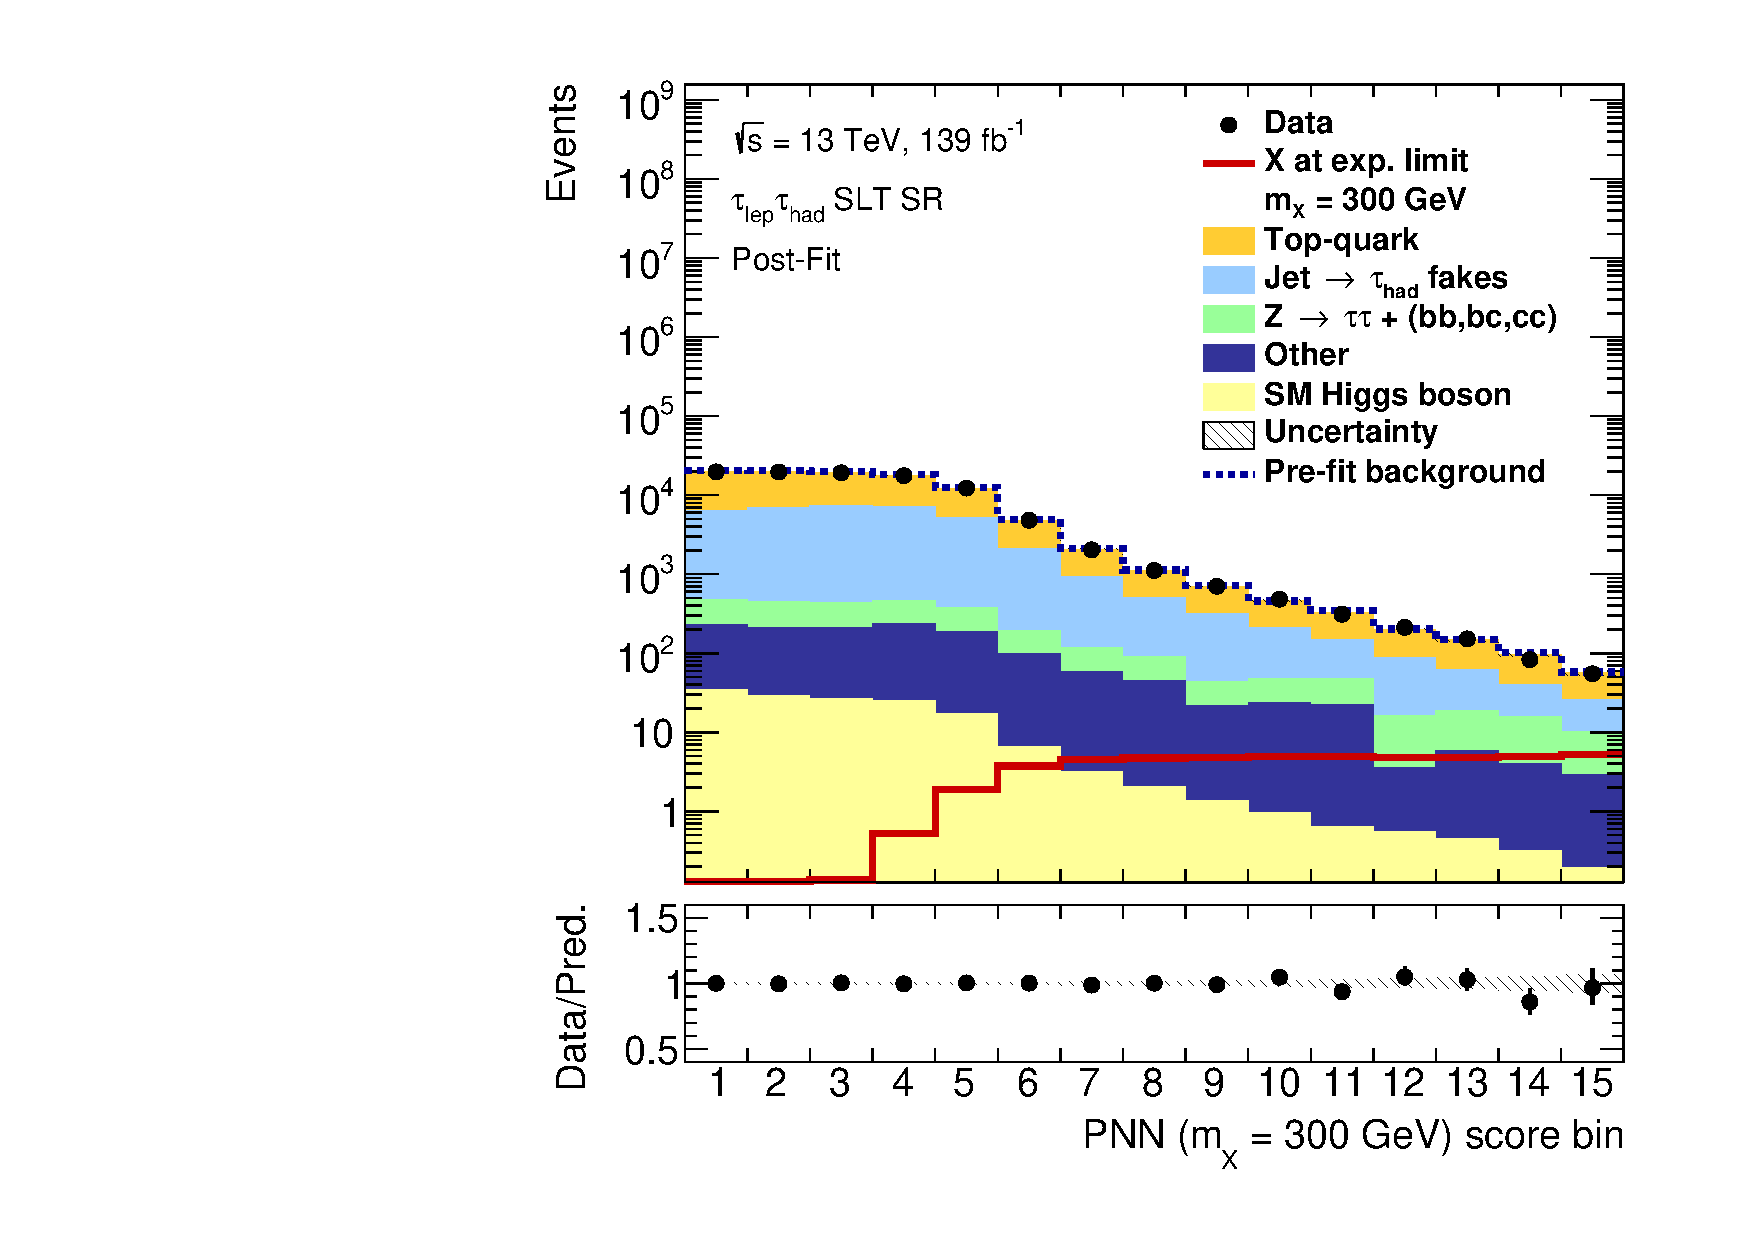
\includegraphics[width=\textwidth]{results_res/postfit/Region_BMin0_incJet1_dist300_J2_D2HDMPNN_T2_SpcTauLH_Y2015_LTT0_L1_GlobalFit_conditionnal_mu0log}
    \subcaption{$\mX = \SI{300}{\GeV}$}
  \end{subfigure}\hfill%
  \begin{subfigure}{0.495\textwidth}
    \centering

    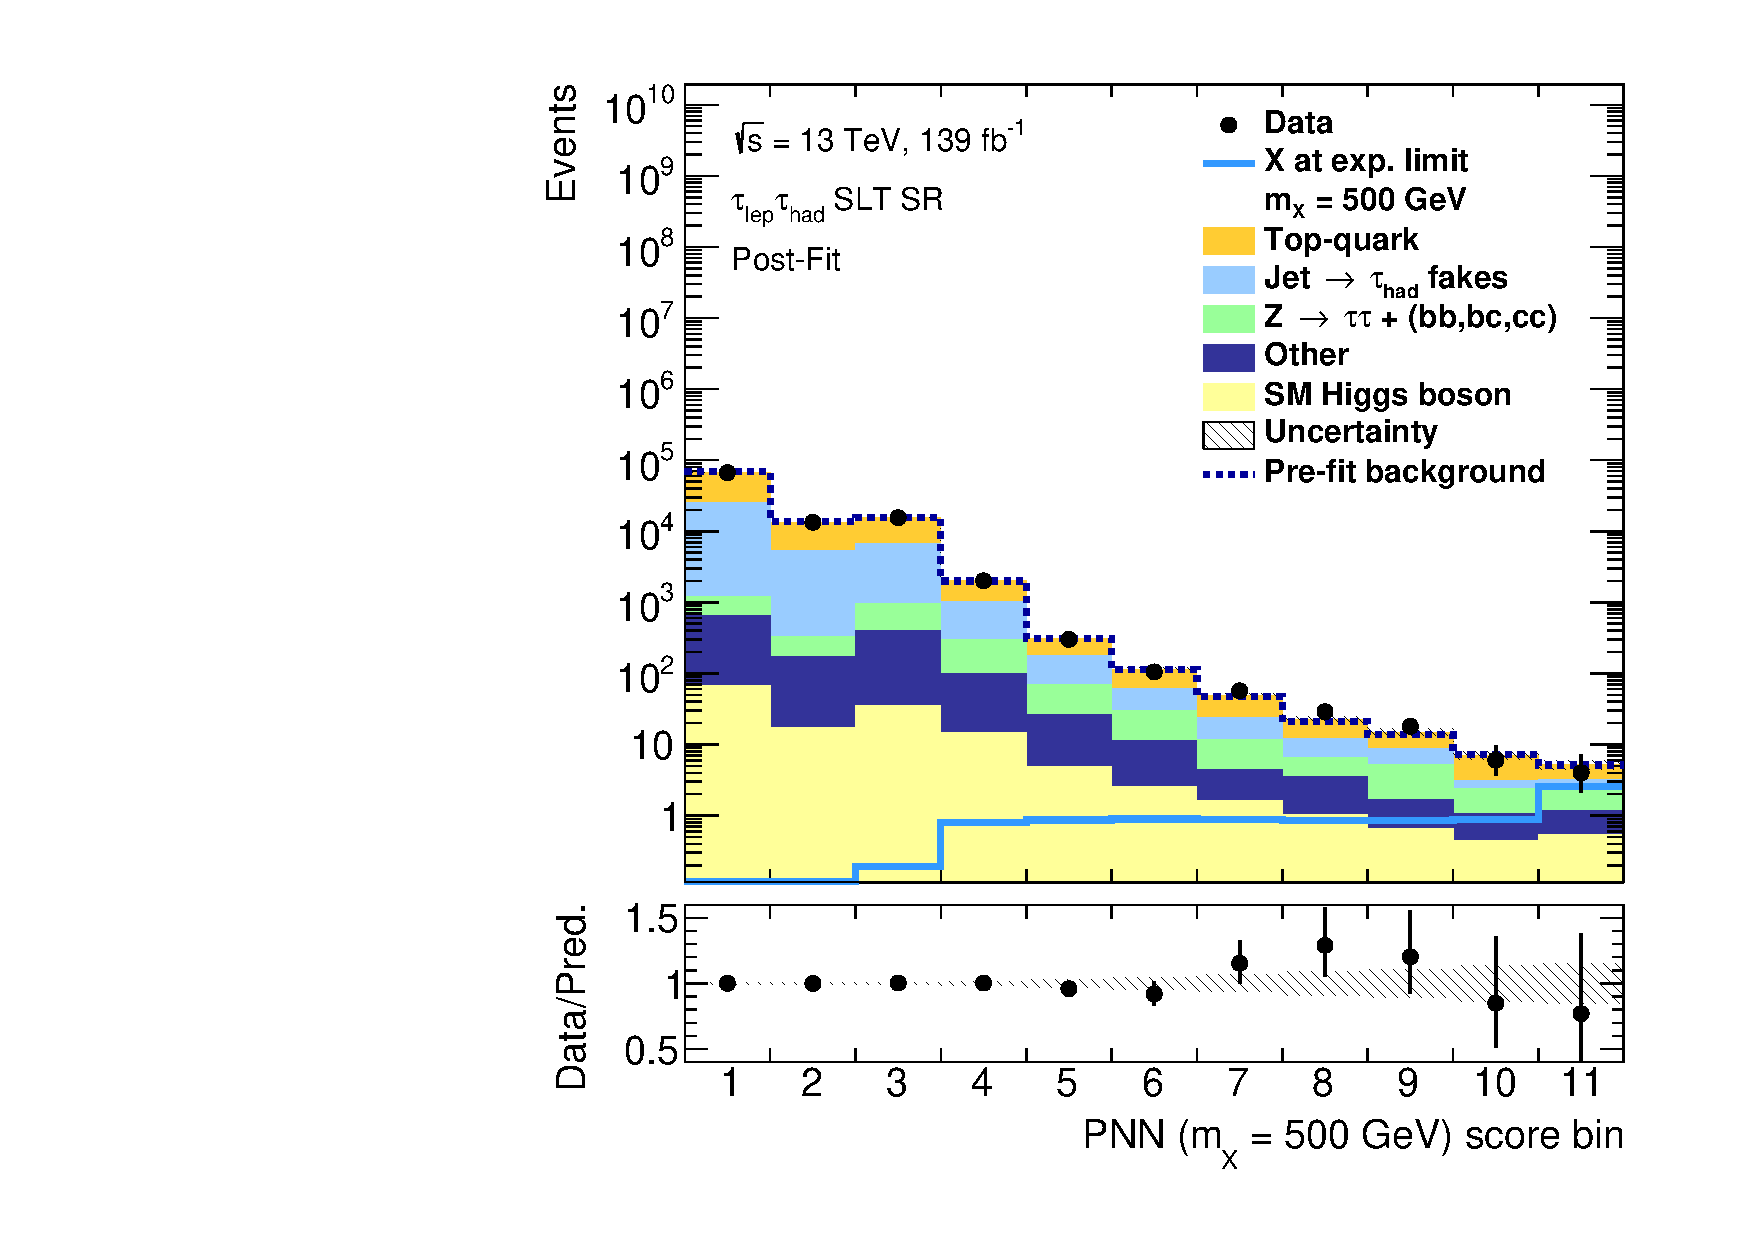
\includegraphics[width=\textwidth]{results_res/postfit/Region_BMin0_incJet1_dist500_J2_D2HDMPNN_T2_SpcTauLH_Y2015_LTT0_L1_GlobalFit_conditionnal_mu0log}
    \subcaption{$\mX = \SI{500}{\GeV}$}
  \end{subfigure}

  \begin{subfigure}{0.495\textwidth}
    \centering

    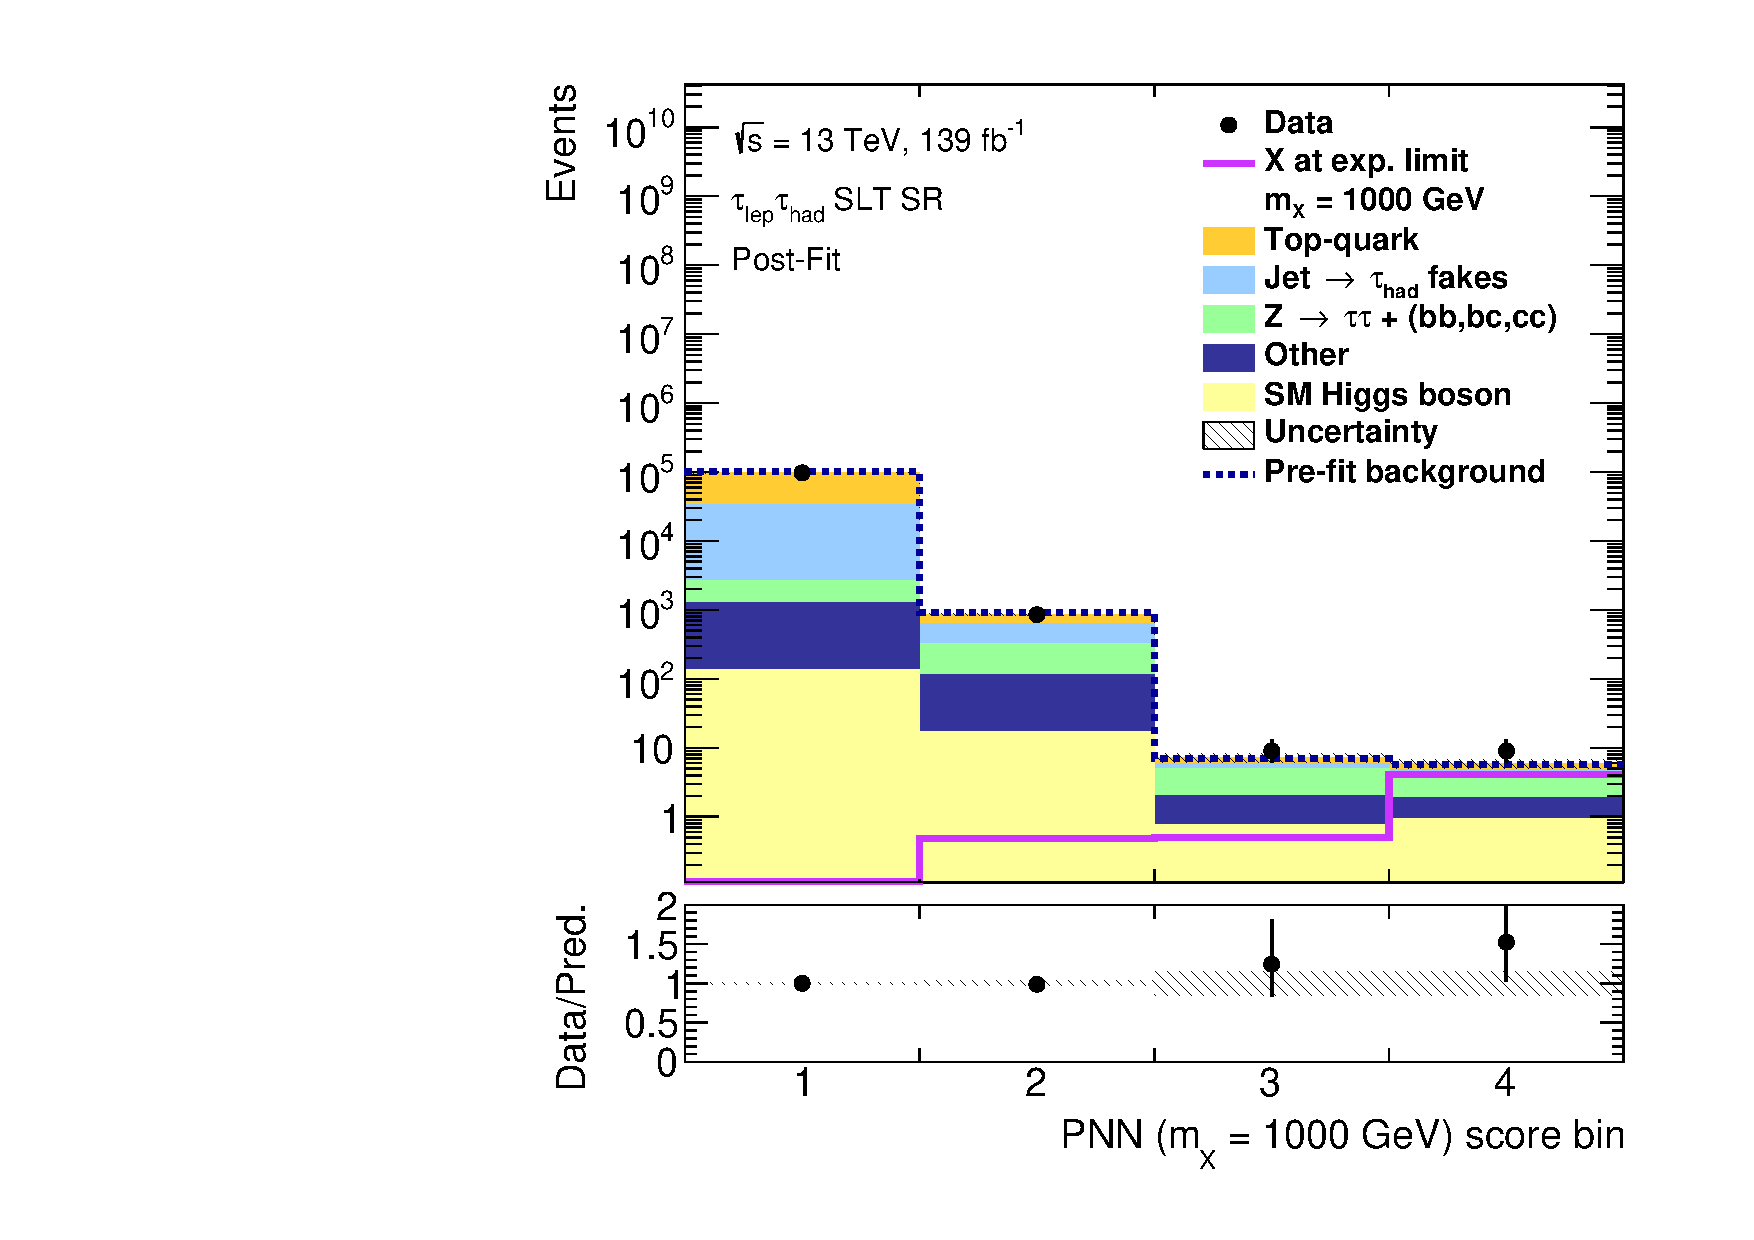
\includegraphics[width=\textwidth]{results_res/postfit/Region_BMin0_incJet1_dist1000_J2_D2HDMPNN_T2_SpcTauLH_Y2015_LTT0_L1_GlobalFit_conditionnal_mu0log}
    \subcaption{$\mX = \SI{1000}{\GeV}$}
  \end{subfigure}\hfill%
  \begin{subfigure}{0.495\textwidth}
    \centering

    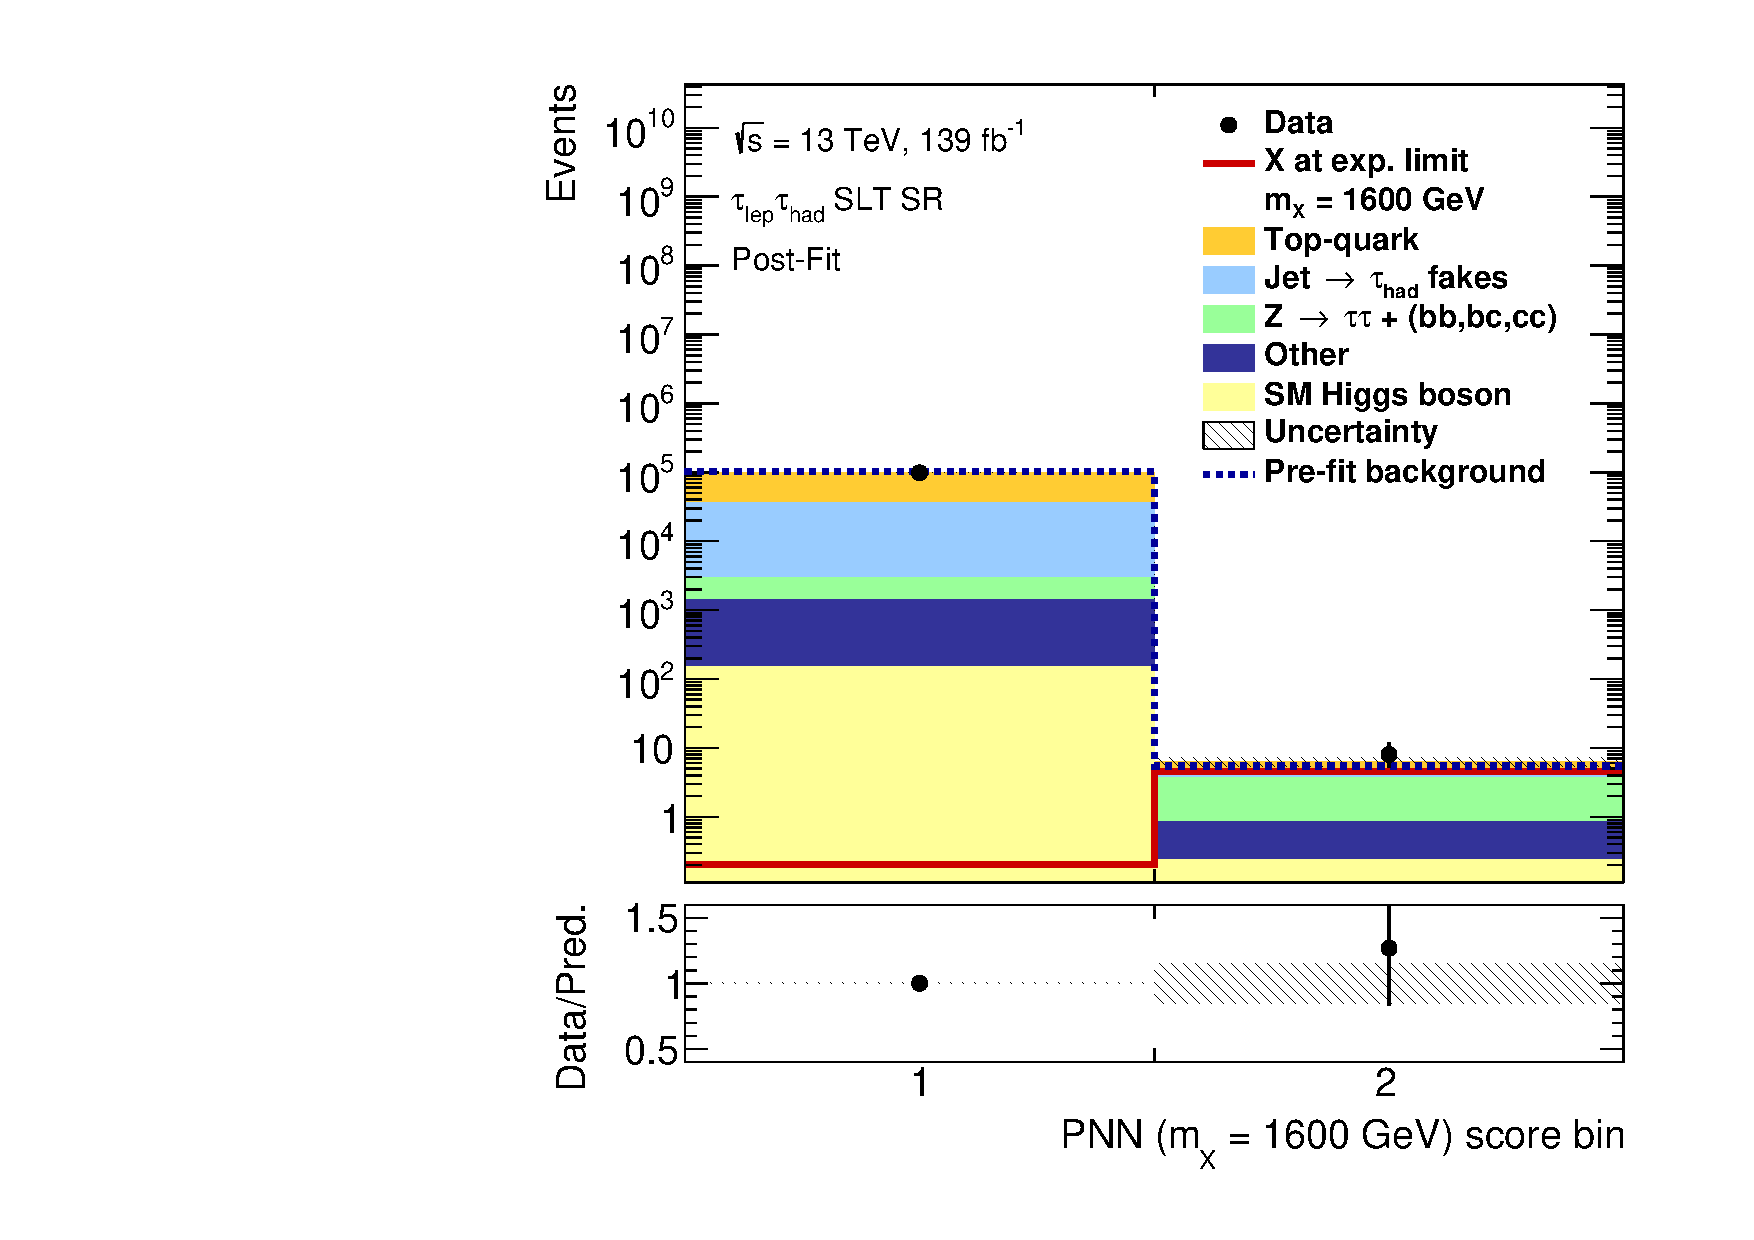
\includegraphics[width=\textwidth]{results_res/postfit/Region_BMin0_incJet1_dist1600_J2_D2HDMPNN_T2_SpcTauLH_Y2015_LTT0_L1_GlobalFit_conditionnal_mu0log}
    \subcaption{$\mX = \SI{1600}{\GeV}$}
  \end{subfigure}

  \caption{Distribution of the PNN discriminant of the \lephad SLT channel after
    the maximum likelihood fit of the background-only model in all SRs and
    CRs. The signal overlay is scaled to the expected upper limit on
    $\sigma(pp \to X \to HH)$.}
\end{figure}


\begin{figure}[htbp]
  \centering

  \begin{subfigure}{0.495\textwidth}
    \centering

    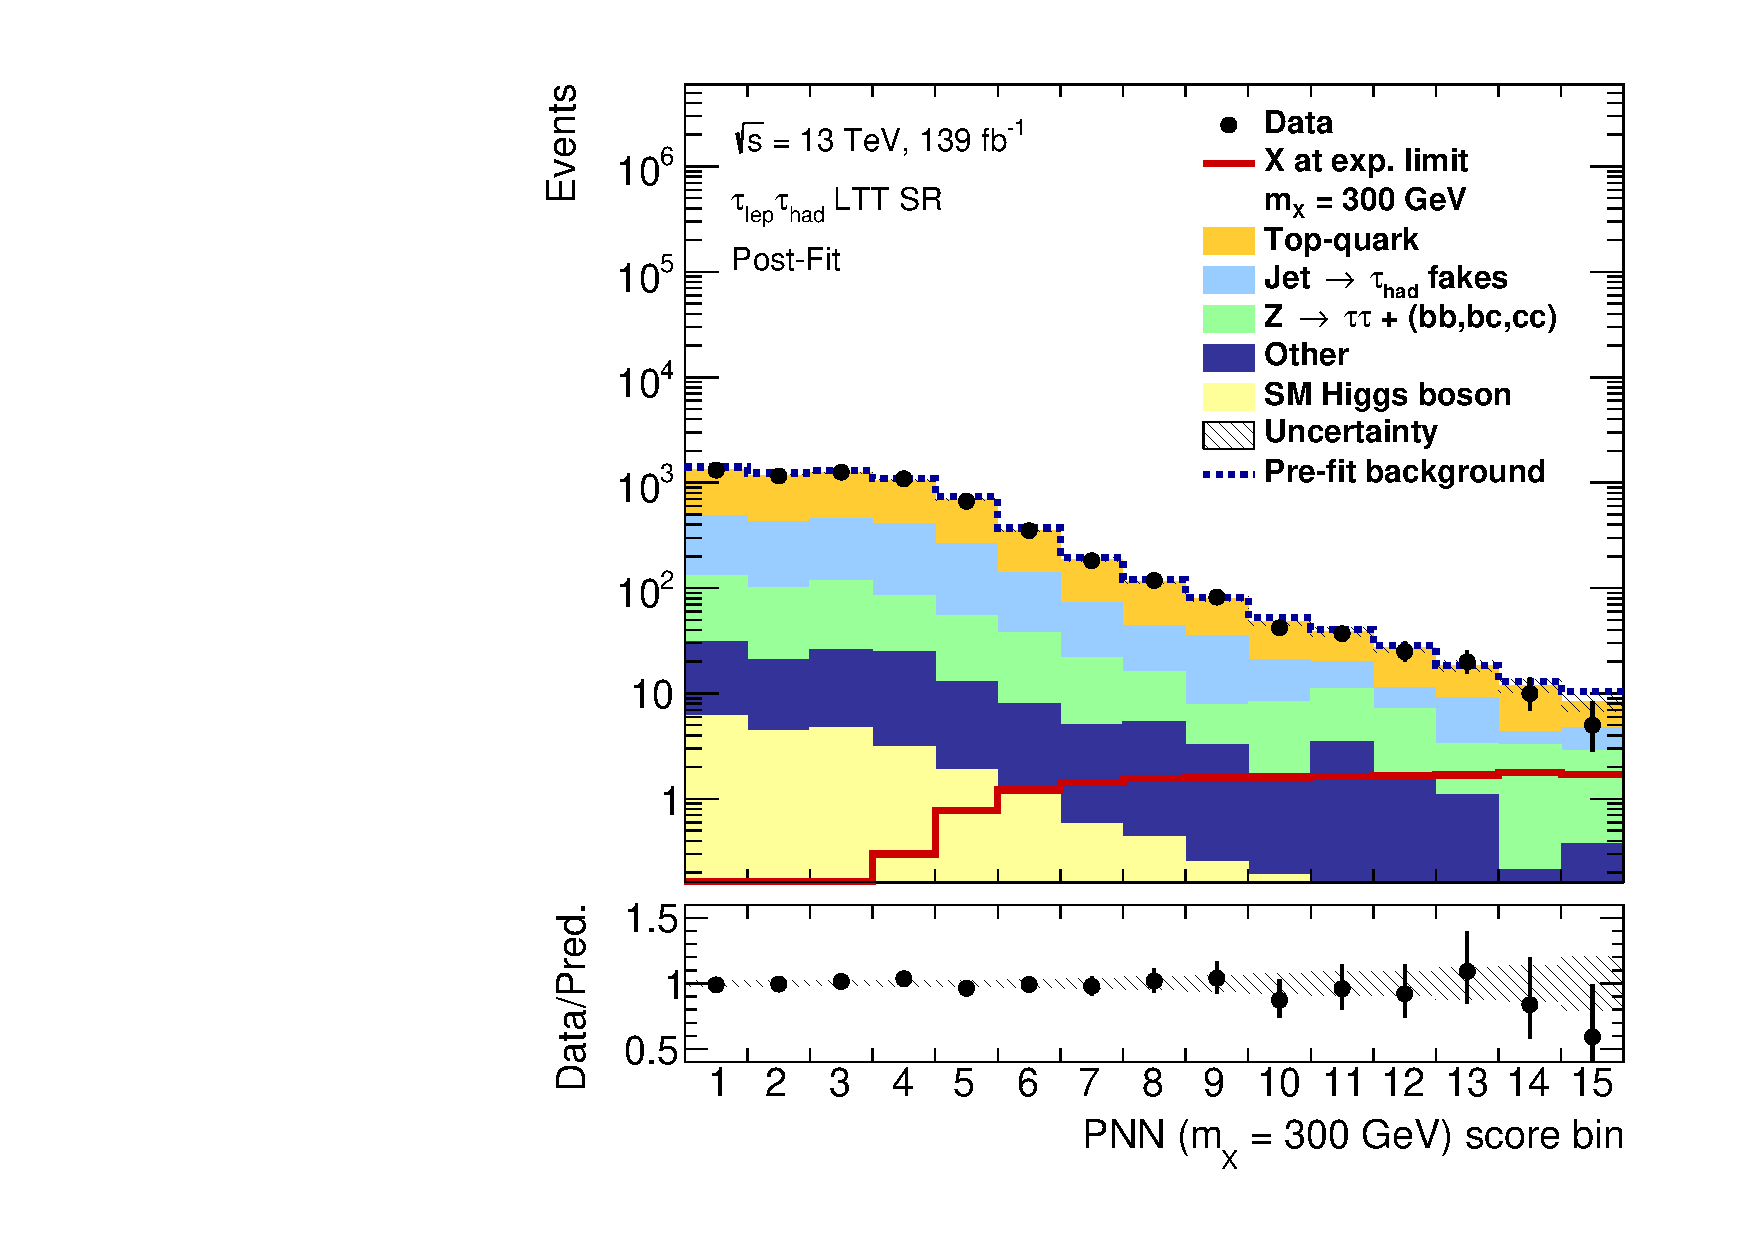
\includegraphics[width=\textwidth]{results_res/postfit/Region_BMin0_incJet1_dist300_J2_D2HDMPNN_T2_SpcTauLH_Y2015_LTT1_L1_GlobalFit_conditionnal_mu0log}
    \subcaption{$\mX = \SI{300}{\GeV}$}
  \end{subfigure}\hfill%
  \begin{subfigure}{0.495\textwidth}
    \centering

    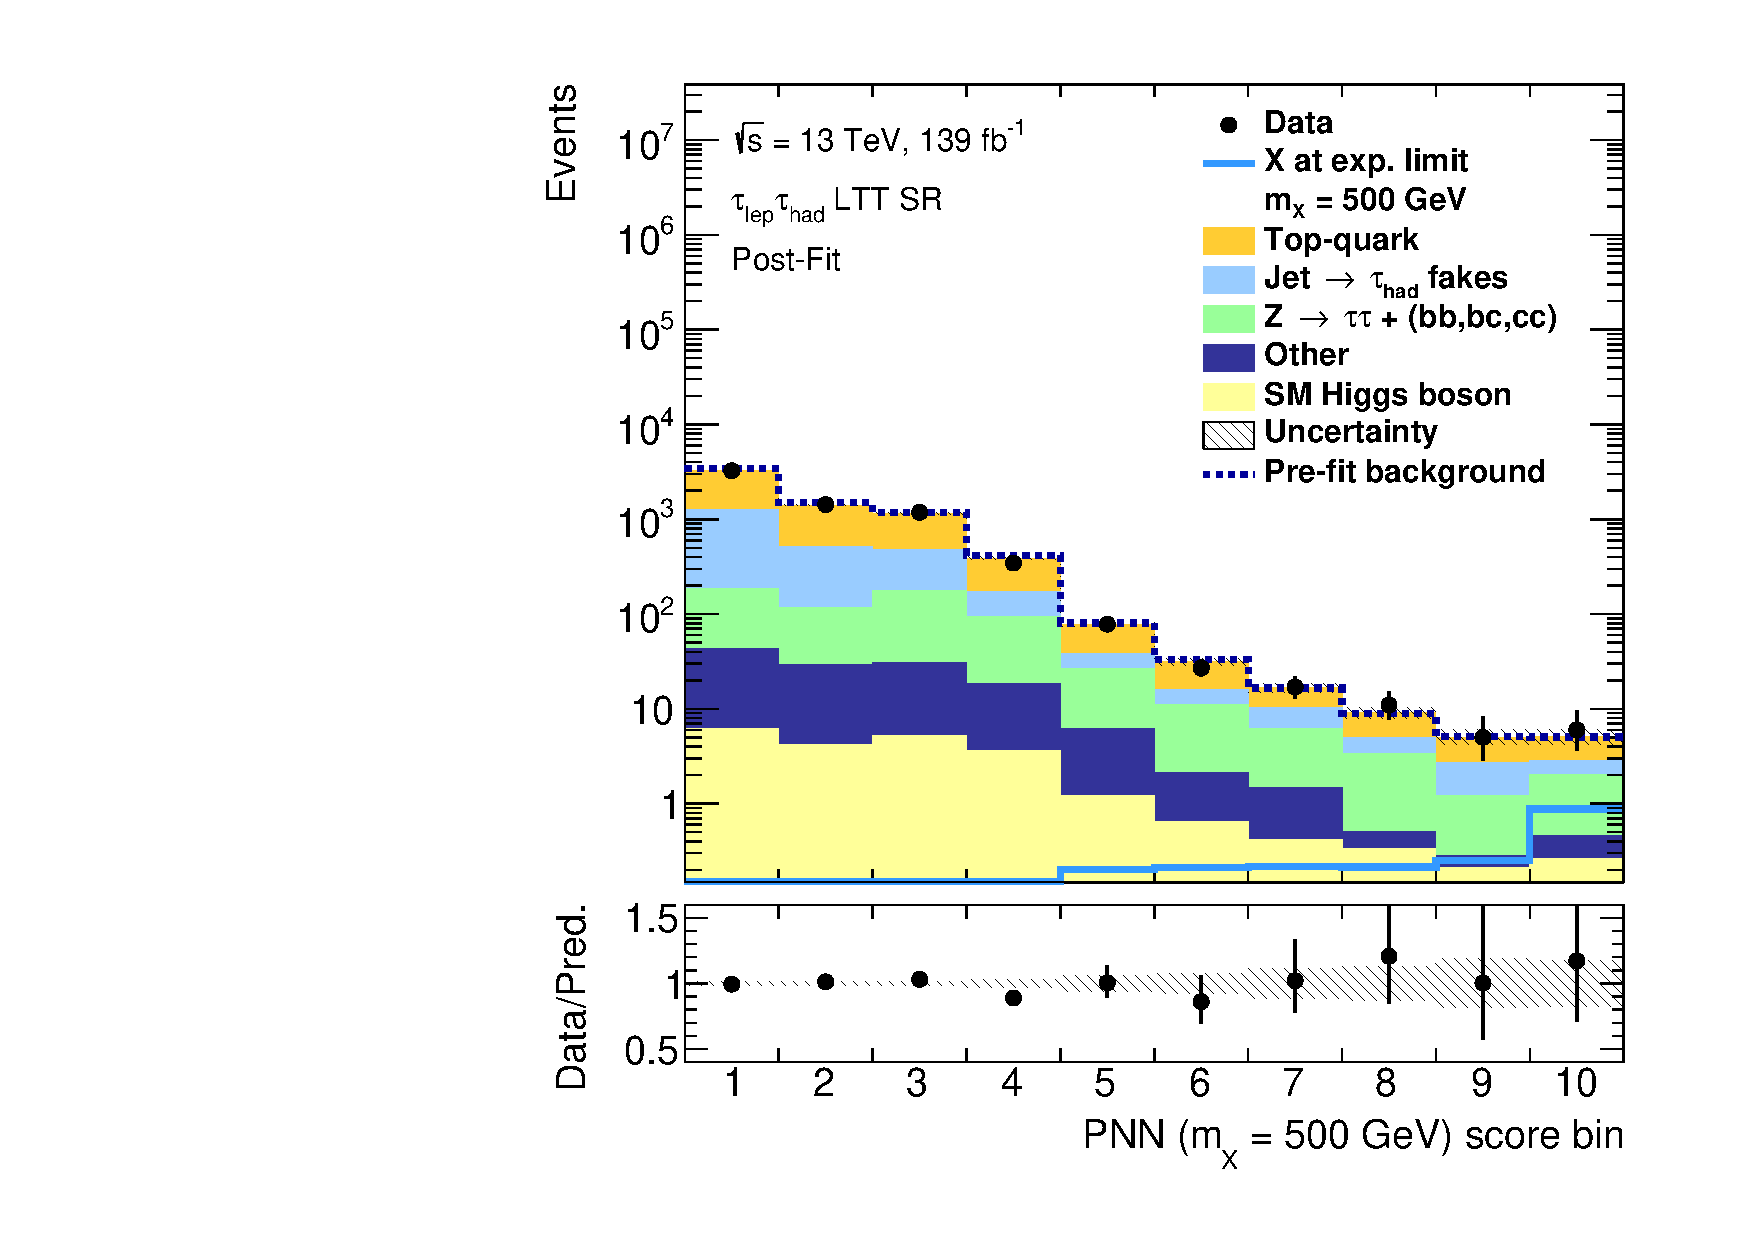
\includegraphics[width=\textwidth]{results_res/postfit/Region_BMin0_incJet1_dist500_J2_D2HDMPNN_T2_SpcTauLH_Y2015_LTT1_L1_GlobalFit_conditionnal_mu0log}
    \subcaption{$\mX = \SI{500}{\GeV}$}
  \end{subfigure}

  \begin{subfigure}{0.495\textwidth}
    \centering

    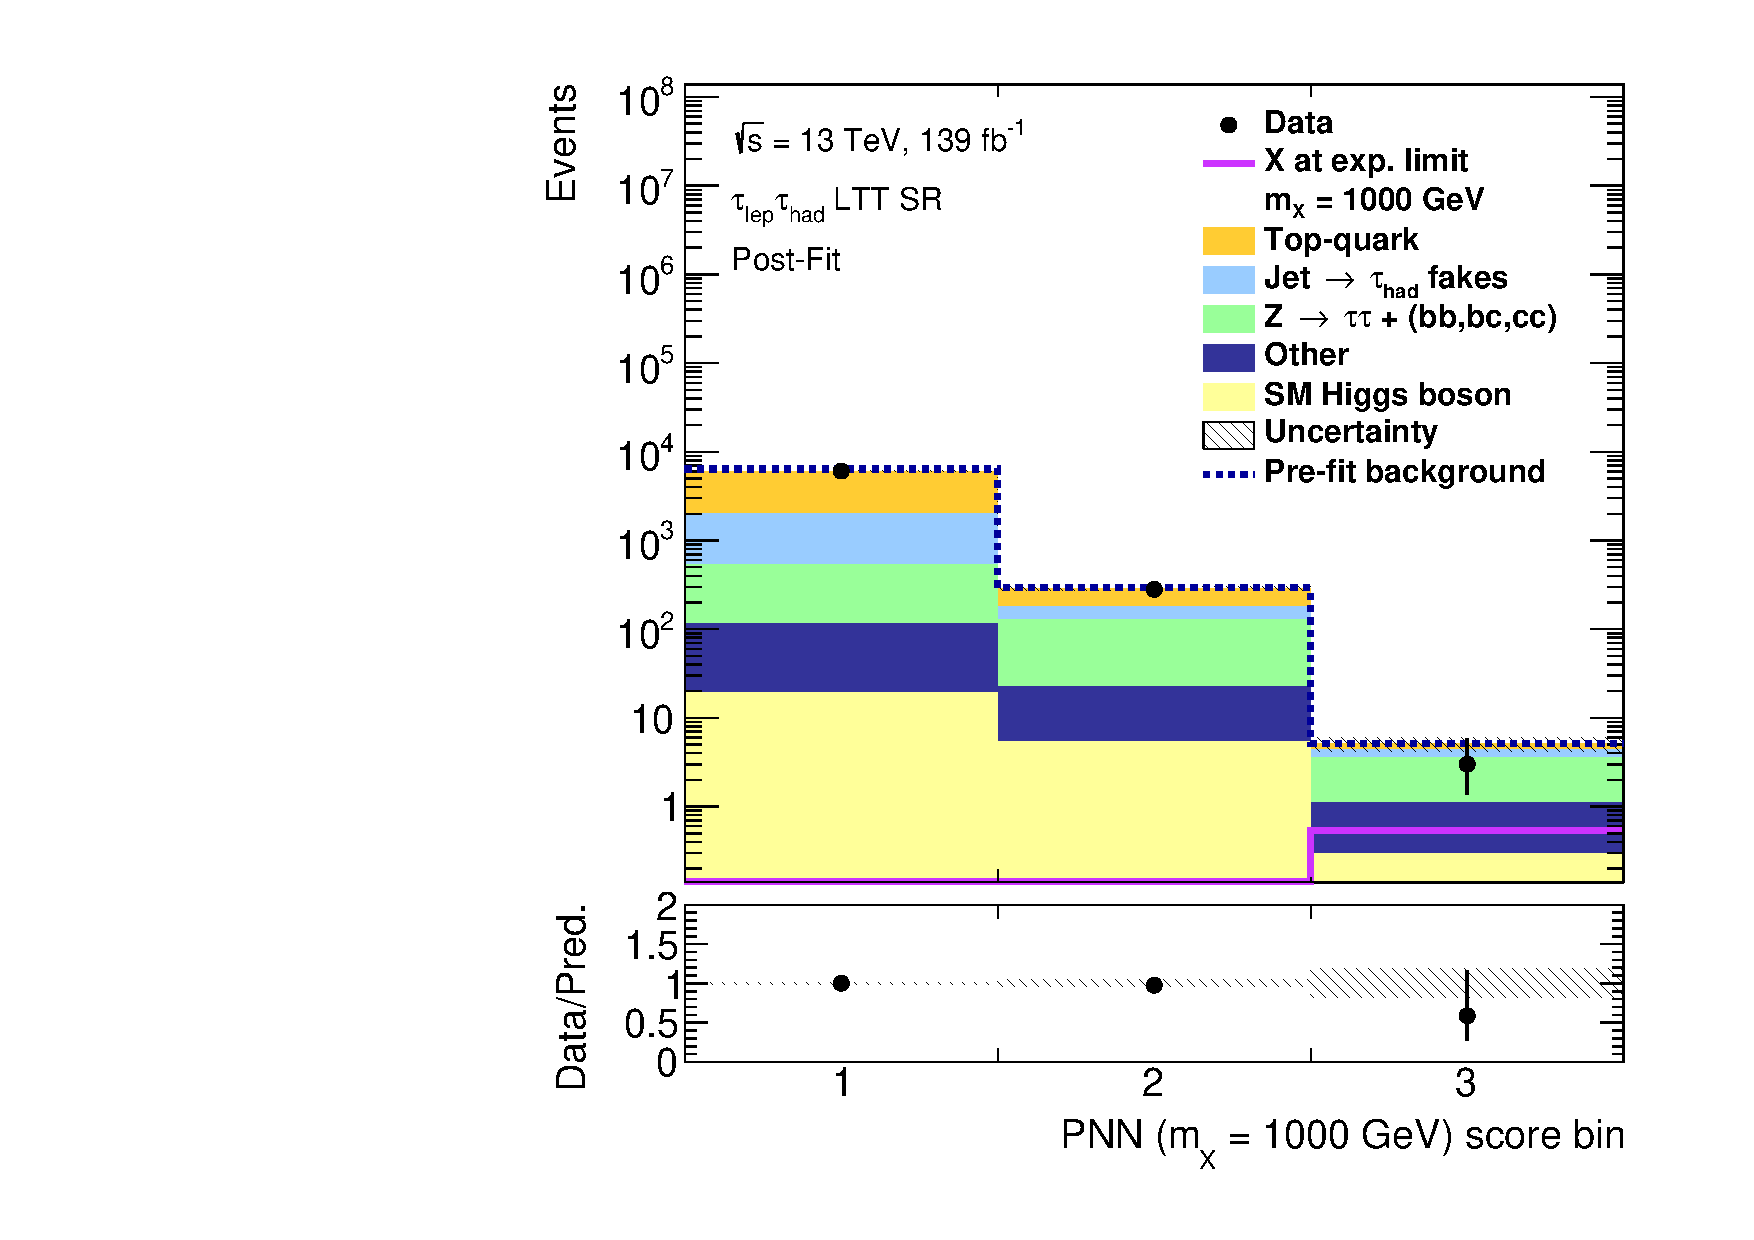
\includegraphics[width=\textwidth]{results_res/postfit/Region_BMin0_incJet1_dist1000_J2_D2HDMPNN_T2_SpcTauLH_Y2015_LTT1_L1_GlobalFit_conditionnal_mu0log}
    \subcaption{$\mX = \SI{1000}{\GeV}$}
  \end{subfigure}\hfill%
  \begin{subfigure}{0.495\textwidth}
    \centering

    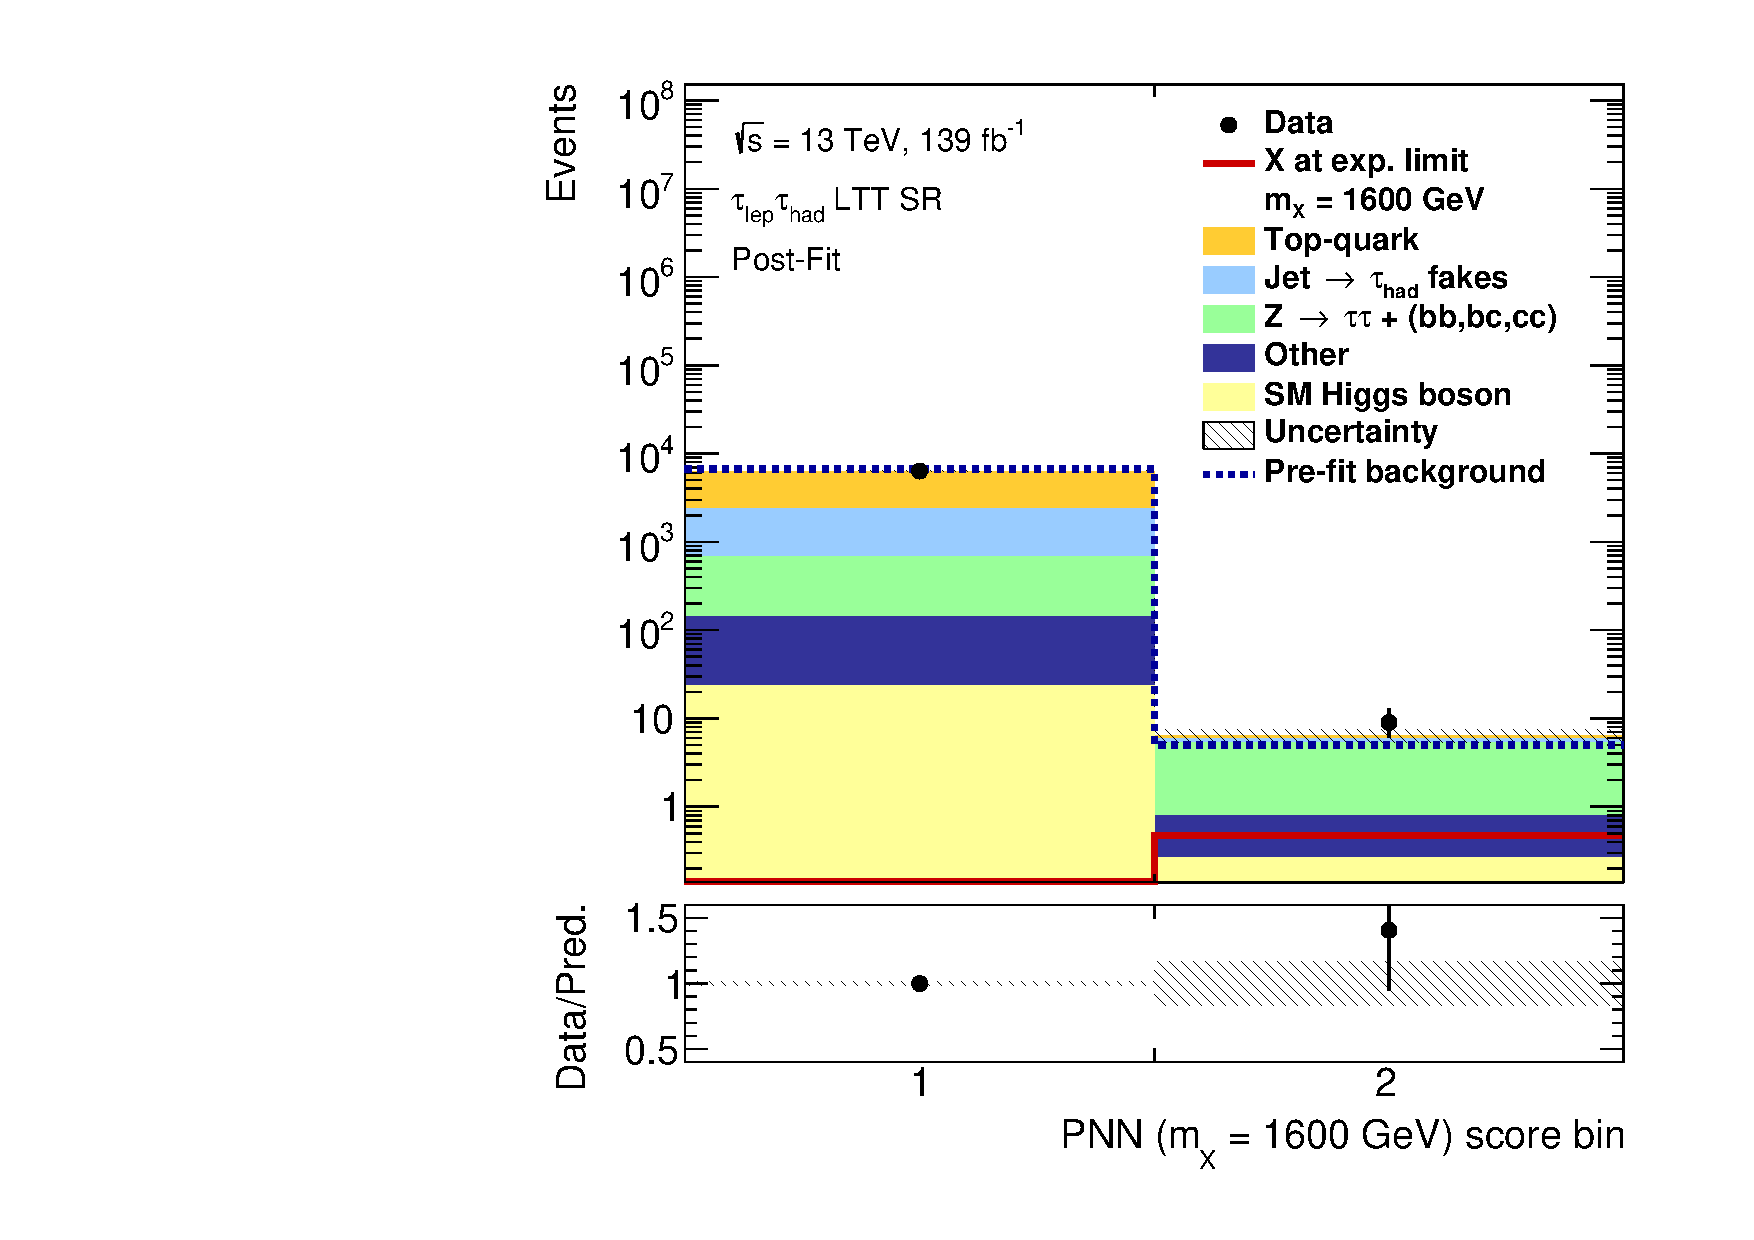
\includegraphics[width=\textwidth]{results_res/postfit/Region_BMin0_incJet1_dist1600_J2_D2HDMPNN_T2_SpcTauLH_Y2015_LTT1_L1_GlobalFit_conditionnal_mu0log}
    \subcaption{$\mX = \SI{1600}{\GeV}$}
  \end{subfigure}

  \caption{Distribution of the PNN discriminant of the \lephad LTT
    channel after the maximum likelihood fit of the background-only
    model in all SRs and CRs. The signal overlay is
    scaled to the expected upper limit on $\sigma(pp \to X \to HH)$.}
\end{figure}


% % ------------------------------------------------------------------------------
% \clearpage
% \subsection{Breakdown}%
% \label{app:breakdown_table}
% % ------------------------------------------------------------------------------

% \begin{table}[htbp]
%   \centering

%   \caption[Breakdown of the variance of $\hat{\sigma}$ by uncertainty category
%   for the search for resonant \HH production.]{Breakdown of the variance on
%     $\hat{\sigma}$, the MLE of the cross section $\sigma(pp \to X\to HH)$, by
%     uncertainty category for the fit to Asimov data with $\mu = 0$ in all
%     regions. The decomposition is determined analogously
%     to~\Cref{tab:breakdown_nonres}.}%
%   \label{tab:breakdown_res_exp_mu0}

%   \begin{tabular}{
  l
  S[table-format=2.0, table-space-text-pre=\textless, table-column-width=1.6cm]
  S[table-format=2.0, table-space-text-pre=\textless, table-column-width=1.6cm]
  S[table-format=2.0, table-space-text-pre=\textless, table-column-width=1.6cm]
  S[table-format=2.0, table-space-text-pre=\textless, table-column-width=1.6cm]
  }
  \toprule
         & \multicolumn{4}{c}{Explained fraction of variance on $\hat{\sigma}$}\\
         %& \multicolumn{4}{c}{of variance on $\hat{\mu}$}\\
  \cmidrule{2-5}
  Source & {$\SI{300}{\GeV}$} & {$\SI{500}{\GeV}$} & {$\SI{1000}{\GeV}$} & {$\SI{1600}{\GeV}$} \\
  \midrule
  \textbf{Data statistical uncertainty}
         & 59\,\si{\percent} & 81\,\si{\percent} & 82\,\si{\percent} & 82\,\si{\percent} \\
  \textbf{Systematic uncertainties}
         & 41\,\si{\percent} & 19\,\si{\percent} & 18\,\si{\percent} & 17\,\si{\percent} \\
  \hspace{0.8em} Instrumental uncertainties
         & 10\,\si{\percent} & 1\,\si{\percent} & 1\,\si{\percent} & {\textless} 1\,\si{\percent}\\
  \hspace{0.8em} Signal modelling uncertainties
         & 1\,\si{\percent}  & 1\,\si{\percent} & {\textless} 1\,\si{\percent} & 3\,\si{\percent} \\
  \hspace{0.8em} Background statistical uncertainties
         & 18\,\si{\percent} & 11\,\si{\percent} & 7\,\si{\percent} & 9\,\si{\percent} \\
  \hspace{0.8em} Background modelling uncertainties
         & 12\,\si{\percent} & 7\,\si{\percent} & 10\,\si{\percent} & 5\,\si{\percent} \\
  \midrule
  \hspace{1.6em} -- \hspace{0.2em} Top-quark (incl.\ free normalisation)
         & 3\,\si{\percent} & 2\,\si{\percent} & 1\,\si{\percent} & {\textless} 1\,\si{\percent} \\
  \hspace{1.6em} -- \hspace{0.2em} \ZHF (incl.\ free normalisation)
         & 3\,\si{\percent} & 1\,\si{\percent} & 3\,\si{\percent} & 2\,\si{\percent} \\
  \hspace{1.6em} -- \hspace{0.2em} SM Higgs boson
         & {\textless} 1\,\si{\percent} & 2\,\si{\percent} & 3\,\si{\percent} & 2\,\si{\percent} \\
  \hspace{1.6em} -- \hspace{0.2em} Fake-\tauhadvis
         & 4\,\si{\percent} & {\textless} 1\,\si{\percent} & 1\,\si{\percent} & 1\,\si{\percent} \\
  \hspace{1.6em} -- \hspace{0.2em} Other
         & {\textless} 1\,\si{\percent} & {\textless} 1\,\si{\percent} & {\textless} 1\,\si{\percent} & {\textless} 1\,\si{\percent} \\
  \bottomrule
\end{tabular}

%%% Local Variables:
%%% mode: latex
%%% TeX-master: "../phd_thesis"
%%% End:

% \end{table}


% ------------------------------------------------------------------------------
\clearpage
\subsection{Nuisance Parameter Pulls and Rankings for the Search for Resonant
  \HH Production}%
\label{app:rankings_resonant}
% ------------------------------------------------------------------------------

\Cref{fig:ranking_pulls_mx300,fig:ranking_pulls_mx500,fig:ranking_pulls_mx1000}


\begin{figure}[htbp]
  \centering

  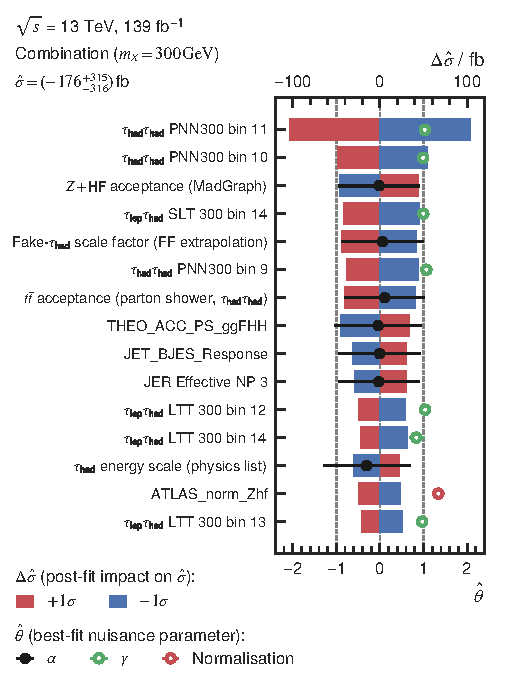
\includegraphics[scale=1.0]{results_res/rankings/ranking_reso_300}

  \caption{Pulls and rankings of NPs in the search for resonant \HH production
    ($\mX = \SI{300}{\GeV}$) after the fit to data in all regions. The best-fit
    cross section for the $\mX = \SI{300}{\GeV}$ signal is
    $\hat{\sigma} =
    (\num{-180}\valuesep^{\hspace{0.25pt}+\hspace{0.25pt}310}_{-320})\valuesep\si{\femto\barn}$.}%
  \label{fig:ranking_pulls_mx300}
\end{figure}


\begin{figure}[htbp]
  \centering

  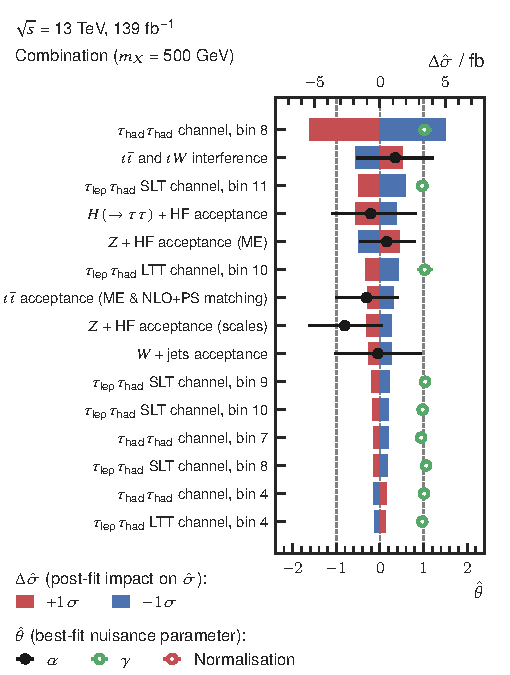
\includegraphics[scale=1.0]{results_res/rankings/ranking_reso_500}


  \caption{Pulls and rankings of NPs in the search for resonant \HH production
    ($\mX = \SI{500}{\GeV}$) after the fit to data in all regions. The best-fit
    cross section for the $\mX = \SI{500}{\GeV}$ signal is
    $\hat{\sigma} =
    (\num{6}\valuesep^{\hspace{0.25pt}+\hspace{0.25pt}20}_{-17})\valuesep\si{\femto\barn}$.}%
  \label{fig:ranking_pulls_mx500}
\end{figure}


\begin{figure}[htbp]
  \centering

  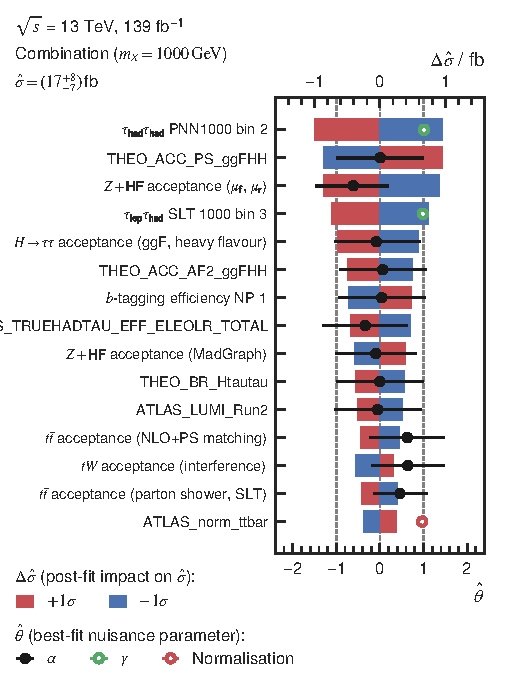
\includegraphics[scale=1.0]{results_res/rankings/ranking_reso_1000}

  \caption{Pulls and rankings of NPs in the search for resonant \HH production
    ($\mX = \SI{1000}{\GeV}$) after the fit to data in all regions. The best-fit
    cross section for the $\mX = \SI{1000}{\GeV}$ signal is
    $\hat{\sigma} =
    (\num{17.4}\valuesep^{\hspace{0.25pt}+\hspace{0.25pt}7.5}_{-6.5})\valuesep\si{\femto\barn}$.}%
  \label{fig:ranking_pulls_mx1000}
\end{figure}


%%% Local Variables:
%%% mode: latex
%%% TeX-master: "../../phd_thesis"
%%% End:
